\begin{graphicspathcontext}{{./chapters/mas/architectures/imgs/},{./chapters/mas/architectures/imgs/auto/},{./chapters/mas/imgs/auto/},\old}

\sidecite{furkranz2011decision, cheung1998using}
\begin{frame}{What is a Decision Tree?}
	\begin{itemize}
	\item Given a set of knowledge, an action may be selected from a set of possible actions
	\item Mapping between inputs and output by sequences of decisions
		\begin{description}
			\item[inputs] part of the knowledge, tested in conditions
			\item[output] zeron one or more actions
		\end{description}
	\end{itemize}
	\begin{columns}
		\begin{column}{.6\linewidth}
			\begin{center}
			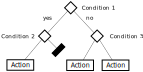
\includegraphics{decisiontree}
			\end{center}
		\end{column}
		\begin{column}{.4\linewidth}
			Complexity: $O(\log_k n)$ \\
			$k$: cardinality of the decision nodes \\
			$n$: number of action nodes
		\end{column}
	\end{columns}
\end{frame}

\begin{frame}[t]{Evaluation Principle}
\begin{itemize}
	\item Start from root decision
	\item For each decision node:
		\begin{enumerate}
			\item Evaluation the condition
			\item Activate the branch according to the condition's value
			\item Select the decision node that is attached to the activated branch
		\end{enumerate}
	\item If an action node is reached, the associated actions are selected
	\item If an iddle node is reached, no action is selected
\end{itemize}
\begin{center}
	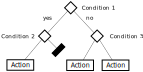
\includegraphics[width=.6\linewidth]{decisiontree}
\end{center}
\end{frame}

\begin{frame}{Types of Decisions}
	\begin{stabularx}{l|X}
		\tabularhead{Condition Type}{Evaluation Principle} \\
		boolean & if true, activate ``yes'' branch, otherwise ``no'' branch \\
		\hline
		enumeration of values & activate the branch associated to the value \\
		\hline
		numeric value & activate the branch associated to a range of values in which the condition value is \\
		\hline
		[3D] vector & activate the branch associated to a range of values in which the vector length is \\
	\end{stabularx}
	
	\hiconbox{Whatever the type of the decisions, they should be simple, i.e. fast to be evaluated}{info-icon}
\end{frame}

\begin{frame}{{Boolean Combination} of Decisions}
	\begin{tabularx}{\linewidth}{XX}
		If C1 \Emph{and} C2 then A1 else A2 & If C1 \Emph{or} C2 then A1 else A2 \\
		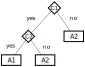
\includegraphics[width=.8\linewidth]{decisiontree_and}
		&
		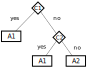
\includegraphics[width=.8\linewidth]{decisiontree_or}
	\end{tabularx}
\end{frame}

\begin{frame}{Knowledge Representation}
	\begin{block}{Direct access to the agent memory}
		\begin{itemize}
			\item Decisions are directly linked to primitive data types
			\item No translation from agent knowledge to decision expressions
		\end{itemize}
	\end{block}
	\begin{alertblock}{Possible Issues}
		\begin{itemize}
			\item Direct access to private data from other characters
			\item Agent implementation-dependent
		\end{itemize}
	\end{alertblock}
	\begin{block}<2>{Possible Solutions}
		To fix these problems, data is insulated inside:
		\begin{itemize}
			\item an enviromnent model, or
			\item a generic agent knowledge representation model.
		\end{itemize}
	\end{block}
\end{frame}

\begin{frame}{Branching Optimization}
	\begin{columns}
		\begin{column}{.5\linewidth}
			\begin{block}{Binary Tree}
				\begin{itemize}
				\item Most decision tree are based on boolean conditions
				\item Easier to optimize (tree balancing)
				\end{itemize}
			\end{block}
			\includegraphics[width=\linewidth]{decisiontree_bin}
		\end{column}
		\begin{column}{.5\linewidth}
			\begin{block}{N-ary Tree}
				\begin{itemize}
				\item Sometimes it is more convenient to have more choices
				\item This structure is flatter:
					\begin{itemize}
						\item only requires one decision
						\item is obviously more efficient
					\end{itemize}
				\end{itemize}
			\end{block}
			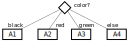
\includegraphics[width=\linewidth]{decisiontree_nary}
		\end{column}
	\end{columns}
\end{frame}

\begin{frame}[fragile]{{Pseudo-Code:} Action}
	\begin{sarllisting}[basicstyle=\scriptsize]
abstract class DecisionTreeNode {
	//Recursively walks through the tree
	abstract def makeDecision
}

abstract class Action extends DecisionTreeNode
	def makeDecision {
		return this
	}
}
	\end{sarllisting}
\end{frame}

\begin{frame}[fragile]{{Pseudo-Code:} Binary Decision}
\begin{sarllisting}[basicstyle=\scriptsize]
abstract class BinaryDecision extends DecisionTreeNode {

	protected var trueNode : DecisionTreeNode

	protected var falseNode : DecisionTreeNode

	protected var testValue : Object

	// carries out the test
	abstract def getBranch : DecisionTreeNode
	
	// Recursively walks through the tree
	def makeDecision {
		// Make the decision and recurse based on the result
		var branch = getBranch
		return branch.makeDecision
	}
}
\end{sarllisting}
\end{frame}

\begin{frame}[fragile]{{Pseudo-Code:} Float Range Decision}
\begin{sarllisting}[basicstyle=\scriptsize]
class FloatBinaryDecision extends BinaryDecision {

	var minValue : float

	var maxValue : float

	def getBranch {
		if ((minValue .. maxValue).contains(testValue as float)) {
			return trueNode
		} else {
			return falseNode
		}
	}
}
\end{sarllisting}
\end{frame}

\begin{frame}[fragile]{{Pseudo-Code:} Multi-Branch Decision}
\begin{sarllisting}[basicstyle=\scriptsize]
class MultiDecision extends DecisionTreeNode {

	var children : List<DecisionTreeNode>

	var testValue : Object
	
	// Carries out the test and returns the node to follow
	def getBranch {
		return children.get(testValue as int)
	}
	
	// Recursively runs the algorithm, exactly as before
	def makeDecision {
		var branch = getBranch
		return branch.makeDecision
	}
}
\end{sarllisting}
\end{frame}

\begin{frame}[t]{Balanced or not?}
	\begin{block}{Unbalanced Tree}
			\begin{center}
				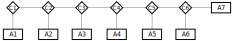
\includegraphics[width=.6\linewidth]{decisiontree_unbalanced}
			\end{center}
		\smaller 
		\begin{tabularx}{\linewidth}{@{}XX@{}}
			Best case: 1 decision & Bad case: 6 decisions \\
			Average case: 4 decisions & Complexity: $O(\frac{n}{2})$ \\
		\end{tabularx}
	\end{block}
	\begin{columns}
		\begin{column}{.5\linewidth}
			\begin{block}{Balanced Tree}
				\begin{tabularx}{\linewidth}{@{}XX@{}}
					\raisebox{-.7\height}{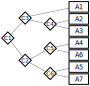
\includegraphics[width=\linewidth]{decisiontree_balanced}} &  \smaller Best: 3 \newline
					Bad: 3 \newline
					Average: 3 \newline
					$O(log_2 n)$
				\end{tabularx}
			\end{block}
		\end{column}
		\begin{column}{.5\linewidth}
			\begin{alertblock}<2>{Balanced or not?}
				\begin{itemize}
					\item Balanced tree $\Rightarrow$ theoretically optimal
					\item What about if C1 is almost always true?
					\item Unbalanced tree becomes the best choice
				\end{itemize}
			\end{alertblock}
		\end{column}
	\end{columns}
\end{frame}

\begin{frame}[t]{Pathological Decision Trees}
	\Emph{Avoiding multiple instances of the same action} \\
	$\Rightarrow$ not assigning an action to more than one leaf
	\begin{center}
		\includegraphics[width=.4\linewidth]{decisiontree_pathologic}
	\end{center}
	\alertbox{Do not introduce loops in the tree}
	\hiconbox{The resulting tree is a \Emph{Directed Acyclic Graph} --- DAG}{info-icon}
\end{frame}

\begin{frame}[t]{{Unrealistic} Random Decision}
	\begin{alertblock}{Problem of Decision Trees}
		If decision trees are \emph{run frequently}, reacting to the immediate state of the world, random decisions cause problems
	\end{alertblock}	
	\begin{example}
		\begin{center}
			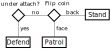
\includegraphics[width=.4\linewidth]{decisiontree_example}
		\end{center}
		\vspace{-.5cm}
		\begin{itemize}
			\item As long as the agent isn't under attack, stand and patrol behaviours will be chosen randomly
			\item This choice is made at every ``frame'', so that the character will appear to vacillate between standing and moving
		\end{itemize}
	\end{example}
\end{frame}

\begin{frame}{{Stability} in Random Choices}
	\alertbox*{Random decision process needs to become \emph{stable}}
	\begin{itemize}
		\item If there is no relevant change in the world state, there should be no change in decision
		\item But, facing the same state at \emph{very different times}, agent can make different decisions
	\end{itemize}
	\begin{block}{Main Principles}
		\begin{itemize}
			\item Allow random decision to keep track of what it did last time
			\item Random selection should be used again after a timeout was reached
		\end{itemize}
	\end{block}
\end{frame}

\end{graphicspathcontext}

\endinput
